
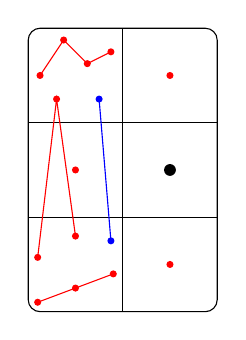
\begin{tikzpicture}[scale=0.6, every node/.style={scale=0.6}]
	\fill (3,3) circle (0.125);
	\fill[red] (1,3) circle (0.075);
	\fill[red] (3,5) circle (0.075);
	\fill[red] (3,1) circle (0.075);
    \draw[rounded corners=1ex] (0,0) rectangle (4,6);
    \draw (0,2) -- (4,2);
    \draw (0,4) -- (4,4);
    \draw (2,0) -- (2,6);
	\coordinate (a1) at (0.2,0.2);
	\coordinate (a2) at (1,0.5);
	\coordinate (a3) at (1.8,0.8);
	\coordinate (b1) at (0.2,1.15);
	\coordinate (b2) at (0.6,4.5);
	\coordinate (b3) at (1,1.6);
	\coordinate (c1) at (0.25,5);
	\coordinate (c2) at (0.75,5.75);
	\coordinate (c3) at (1.25,5.25);
	\coordinate (c4) at (1.75,5.5);
	\coordinate (d1) at (1.5,4.5);
	\coordinate (d2) at (1.75,1.5);
	\fill[red] (a1) circle (0.075);
	\fill[red] (a2) circle (0.075);
	\fill[red] (a3) circle (0.075);
	\fill[red] (b1) circle (0.075);
	\fill[red] (b2) circle (0.075);
	\fill[red] (b3) circle (0.075);
	\fill[red] (c1) circle (0.075);
	\fill[red] (c2) circle (0.075);
	\fill[red] (c3) circle (0.075);
	\fill[red] (c4) circle (0.075);
	\fill[blue] (d1) circle (0.075);
	\fill[blue] (d2) circle (0.075);
	\draw[red] (a1) -- (a2) -- (a3);
	\draw[red] (b1) -- (b2) -- (b3);
	\draw[red] (c1) -- (c2) -- (c3) -- (c4);
	\draw[blue] (d1) -- (d2);
\end{tikzpicture}
\begin{tikzpicture}[scale=0.6]
	\draw[white] (0,0) rectangle (2,6);
	\draw[thick, ->] (-.5,3) -- (2.5,3) node[above,pos=.5] {$\textsf{rev}_{[0,0]}$};
\end{tikzpicture}
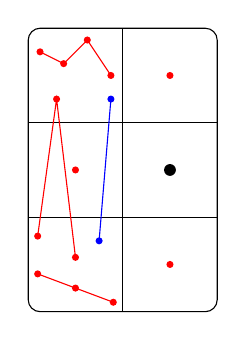
\begin{tikzpicture}[scale=0.6, every node/.style={scale=0.6}]
	\fill (3,3) circle (0.125);
	\fill[red] (1,3) circle (0.075);
	\fill[red] (3,5) circle (0.075);
	\fill[red] (3,1) circle (0.075);
    \draw[rounded corners=1ex] (0,0) rectangle (4,6);
    \draw (0,2) -- (4,2);
    \draw (0,4) -- (4,4);
    \draw (2,0) -- (2,6);
	\coordinate (a1) at (1.8,0.2);
	\coordinate (a2) at (1,0.5);
	\coordinate (a3) at (0.2,0.8);
	\coordinate (b1) at (1,1.15);
	\coordinate (b2) at (0.6,4.5);
	\coordinate (b3) at (0.2,1.6);
	\coordinate (c1) at (1.75,5);
	\coordinate (c2) at (1.25,5.75);
	\coordinate (c3) at (0.75,5.25);
	\coordinate (c4) at (0.25,5.5);
	\coordinate (d1) at (1.75,4.5);
	\coordinate (d2) at (1.5,1.5);
	\fill[red] (a1) circle (0.075);
	\fill[red] (a2) circle (0.075);
	\fill[red] (a3) circle (0.075);
	\fill[red] (b1) circle (0.075);
	\fill[red] (b2) circle (0.075);
	\fill[red] (b3) circle (0.075);
	\fill[red] (c1) circle (0.075);
	\fill[red] (c2) circle (0.075);
	\fill[red] (c3) circle (0.075);
	\fill[red] (c4) circle (0.075);
	\fill[blue] (d1) circle (0.075);
	\fill[blue] (d2) circle (0.075);
	\draw[red] (a1) -- (a2) -- (a3);
	\draw[red] (b1) -- (b2) -- (b3);
	\draw[red] (c1) -- (c2) -- (c3) -- (c4);
	\draw[blue] (d1) -- (d2);
\end{tikzpicture}